\label{sec:IF_MicroBooNE}
The MicroBooNE experiment is the first detector deployed at the SBN facility and represents the next step in LArTPC technology. It is a 10.3~m~$\times$~2.5~m~$\times$~2.3~m TPC with 89 tons of active volume. The TPC has three instrumented wire planes with the first two induction planes oriented at $\pm 30^{\circ}$ to the beam axis and the third plane oriented vertically. Both the pitch and wire spacing are chosen to be 3~mm, which provide a superb resolution for imaging interactions inside the detector. Additionally there are thirty two 8'' cryogenic photomultiplier tubes (PMTs) which provide the $t_{0}$ for an interaction by recording the scintillation light produced when the charged particles interact in LAr. In the summer of 2015 MicroBooNE was filled with LAr and began commissioning.  With the rapid success of the system, MicroBooNE has been taking neutrino data starting October, 2015. Figure \ref{fig:uboone} shows an event display of an automatically identified neutrino candidate event collected by utilizing both light and charge information. 

\begin{figure}[htb]
\centering
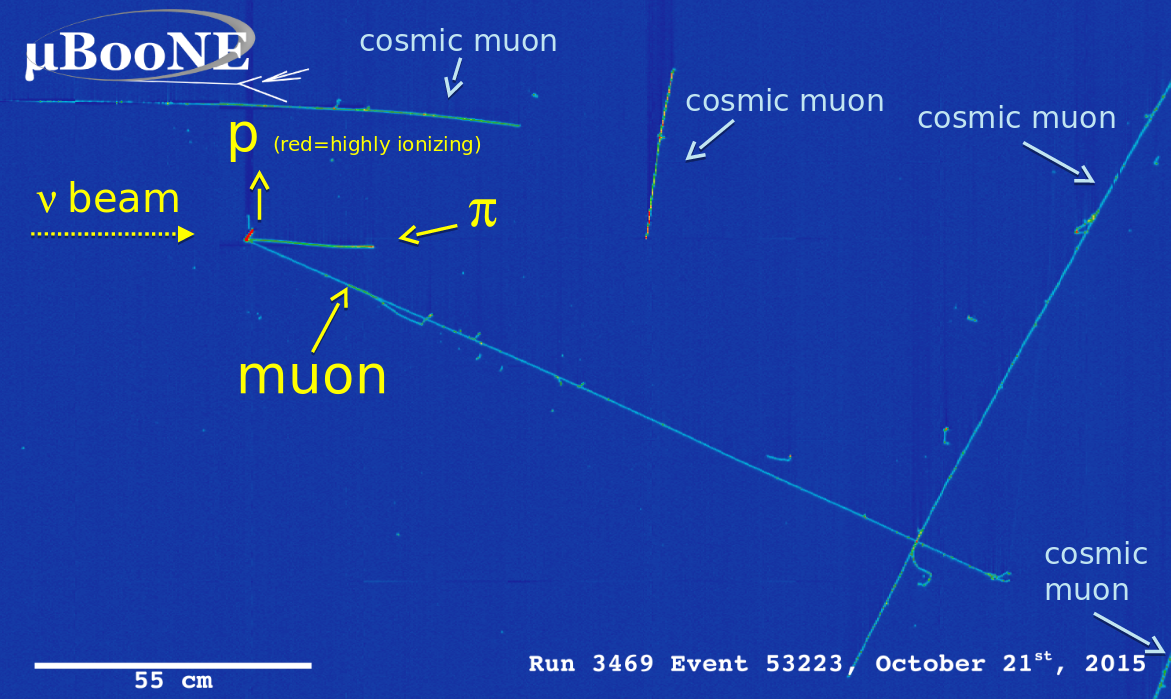
\includegraphics[width=0.55\textwidth]{images/ubooneNeutrino.png}
\caption[]{Event display of an automatically identified neutrino interaction utilizing the light and charge readout in MicroBooNE.}
\label{fig:uboone}
\end{figure}

One of the most compelling measurements MicroBooNE will make is to confirm or refute the nature of the MiniBooNE low-energy electron neutrino excess. Utilizing the particle identification powers of the LArTPC (specifically the dE/dX discrimination), MicroBooNE will be able to differentiate the electron-like electromagnetic showers from those photon-like. Moreover, the dominant background in the MiniBooNE analysis, NC$-\pi^{0}$ production can be significantly reduced using the powerful imaging techniques of a LArTPC. The analysis techniques for the low energy excess search will be developed in the common software framework LArSoft. Since LArSoft is designed to be common use of LArTPC experiments, the reconstruction techniques and analysis strategies developed on MicroBooNE will have direct applicability to other LArTPC experiments.

MicroBooNE will also be able to measure many high-statistic cross-sections at $E_{\nu} < 1$GeV. At this energy range, the impact of various nuclear effects such as final state interactions and short-range nucleon correlation are poorly understood. These nuclear effects can change the classification of neutrino-nucleus ($\nu-n$) interaction, and thus change the measured cross-section. The fine grain tracking offered by LArTPCs allows for the classification of $\nu-n$ interaction in terms of final state particles instead of using simplifications such as the quasi-elastic scattering assumption. Moreover, with a proton threshold measured as low as 21~MeV of kinetic energy \cite{Argoneut}, these nuclear effects can be measured with high statistics using neutrinos as a probe. The broader neutrino cross-section community is anticipating how MicroBooNE results compare to previous measurements.

Asaadi will be the only P.I. on this experiment.

%MicroBooNE will also explore the physics capabilities of LArTPC including classification of low energy events as a background for supernova neutrinos and searching for cosmogenic backgrounds related to proton decay analysis. While MicroBooNE is too small and located on the surface making meaningful proton decay search impossible. However, utilizing the abundance of cosmic rays to search for background signatures due to cosmogenic sources can provide useful input to future analysis targeted at the Deep Underground Neutrino Experiment (DUNE). Fully exploring the physics capabilities of the MicroBooNE detector enables a robust physics program. 

%%%%%%%%%%%%%%%%%%%%%%%%%%%%%%%%%%%%%%%%%%%%%%%%%%%%%%%%%%%%%%%%%%%%%
\subsubsection{MicroBooNE Operations}\label{sec:UbooneOperations}
%%%%%%%%%%%%%%%%%%%%%%%%%%%%%%%%%%%%%%%%%%%%%%%%%%%%%%%%%%%%%%%%%%%%%
Asaadi will continue to play a major role in the data taking and operations of the MicroBooNE detector.  He has served as the TPC commissioning leader and now as the TPC operations expert. Asaadi has only recently stepped down as Astro-Particle and Exotics working group convener, but remains active in this group for the foreseeable future where a natural synergy exists within the UTA group given Yu's role as a DUNE BSM co-onvener. MicroBooNE will explore the physics capabilities of LArTPC including classification of low energy events as a background for supernova neutrinos and searching for cosmogenic backgrounds related to proton decay analysis.

One post-doctoral researcher supported by the funds requested in this proposal will spend part of his/her time working on the MicroBooNE operations and is expected to be trained to serve as the TPC operations expert. This is in addition to the efforts expected from the postdoc supported by Asaadi's start-up funds in the first two years of this proposal.  Besides the data taking shift requirements, he/she is also expected to play a role in the online DAQ/data quality management as a training for the planned work on the SBND DAQ described in the previous section. With MicroBooNE just finishing the commissioning of their continuous readout data stream (``supernova data stream''), UTA will be able to play a role in supporting the analysis and further improvement of this system. The graduate student supported by this proposal is also expected to take shifts on MicroBooNE and participate in the expert training. While stationed at UTA, graduate and undergraduate students will take remote shifts on this experiment utilizing UTA's remote shift station described earlier. 


%%%%%%%%%%%%%%%%%%%%%%%%%%%%%%%%%%%%%%%%%%%%%%%%%%%%%%%%%%%%%%%%%%%%%
\subsection{MicroBooNE Data Analysis}\label{sec:UbooneDataAnalysis}
%%%%%%%%%%%%%%%%%%%%%%%%%%%%%%%%%%%%%%%%%%%%%%%%%%%%%%%%%%%%%%%%%%%%%
Being a driving force on early neutrino cross-section analysis is a good way to have impact on the physics program at MicroBooNE. The postdoctoral researchers and the graduate student are expected to work on neutrino cross-section analysis using the early data in addition to the measurements done once the full SBN program is operational. This data set will provide first glimpses into the short-baseline analysis. Following up on previous low statistics cross-sections measured by ArgoNeuT is one way which UTA can have immediate impact and leverage previous experience through Asaadi's major role. 

An example of one such cross-section measurement of immediate interest, shown in Figure \ref{fig:cccohpion} is the charged current coherent charged pion production (CC Coh-$\pi$). This result is of particular interest since it is an example of a relatively simple topology, but one where theory and experiment do not agree. Previous attempts to measure this cross-section at low energy by the SciBooNE and K2K collaborations have been unsuccessful. On the other hand, the analogous neutral current process (NC Coh-$\pi^{0}$)has been observed at low energy. To further complicate this picture, two higher energy measurements from ArgoNeuT and Minerva both show observation of CC Coh-$\pi$ although somewhat at odds with various modern neutrino generator predictions. In this regard, the initial MicroBooNE data set will be a valuable tool in disentangling this issue and many other cross-section oddities and allow for a better construction of $\nu$-Ar scattering models. Researchers from UTA are expected to play a leading role in the analysis of CC Coh-$\pi$ data sample in MicroBooNE and begin exploration of the NC Coh-$\pi$ production. This analysis is expected to build on the work began in ArgoNeuT \cite{Argoneut} and builds on the groups expertiese for charged pion identification developed through the work in LArIAT.
 
\begin{figure}[htb]
\centering
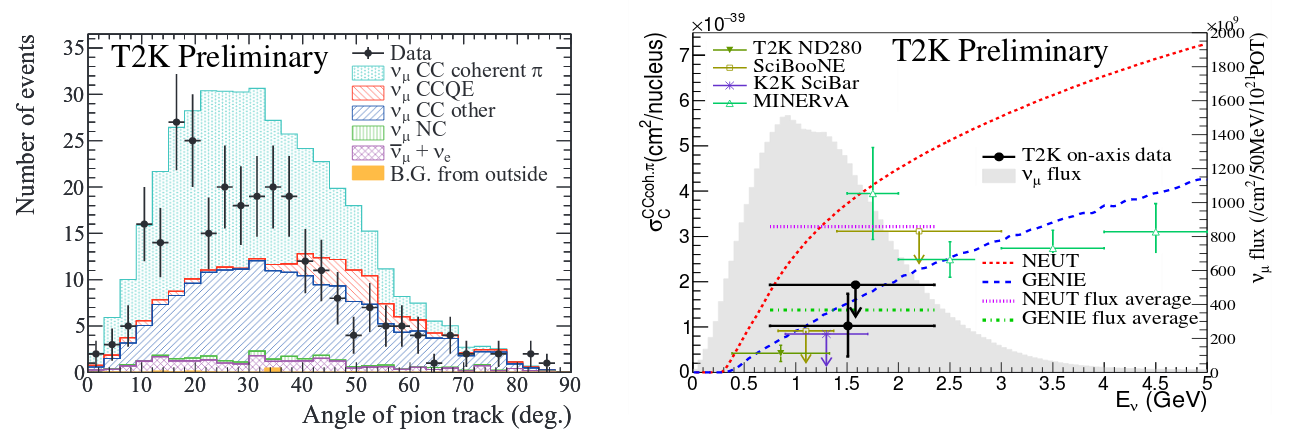
\includegraphics[width=0.98\textwidth]{images/CCCohPion.png}
\caption[]{Recent results from T2K \cite{T2K} showing the tension which exists from the low-energy and high energy measurements of the cCC Coh-$\pi$ production. With the SciBooNE and K2K experiments showing no evidence of this process at $E_{\nu} < 1$ GeV but ArgoNeuT and Minerva both measuring this process at higher energy. Moreover, the recent results from T2K disagree with the current cross-section models.}
%Need to cite as http://www.t2k.org/docs/proc/056/jpsaccepted
\label{fig:cccohpion}
\end{figure}


The tools developed for data analysis and reconstruction in MicroBooNE will have transferability to the other SBN LArTPC experiments through the use of the common software package, LArSoft. UTA group has developed expertise on LArSoft with Asaadi contributing to the development and planning of it and will continue to contribute to its further development as a tool to perform a synthesized analysis across the SBN.
